\documentclass[a4paper,arial,10pt]{article}
\usepackage[spanish]{babel}
\usepackage{tkz-berge}
\usepackage[pdftex]{graphicx}
\usepackage{sagetex}
\usepackage{verbatim}   % useful for program listings
\usepackage{color}      % use if color is used in text
\usepackage{subfigure}  % use for side-by-side figures
\usepackage{xy}         % XY-pic diagrams are drawn over a matrix-oriented canvas, where each diagram element is placed in a matrix slot.
\usepackage[pdftex,bookmarks,colorlinks]{hyperref}   % use for hypertext links, including those to external documents and URLs
\usepackage{float}
\usepackage{wrapfig}
\usepackage{textcomp}
\usepackage[T1]{fontenc}
\usepackage{pxfonts}
\pagestyle{empty}
\renewcommand{\rmdefault}{phv} % Arial
\renewcommand{\sfdefault}{phv} % Arial
\usepackage{anysize}
\usepackage{lscape}
\marginsize{2cm}{2cm}{2cm}{2cm}

\begin{document}
\begin{sagesilent}
MIARCHIVO = "glass_ymax_short_fixed_at_12v_06v_to_4v.txt"
#solo el nombre no hace falta la direccion

from loaddb import myDB
import pylab

values = myDB.get_original_data(MIARCHIVO)
std, slope, intercept, r_value, p_value = myDB.get_lineal_regression(MIARCHIVO)

pylab.plot(values[0], values[1], '-')
pylab.plot(values[0], [intercept + slope*x  for x in values[0]], 'r-')
pylab.xlabel('Number of ....')

#pylab.xlim(xmin=0.0000000, xmax=-0.5)
#pylab.ylim(ymin=0.0000000, ymax=-0.2) 

pylab.savefig("../plots/test.png", dpi = 80)


\end{sagesilent}

\begin{figure}
\begin{center}
        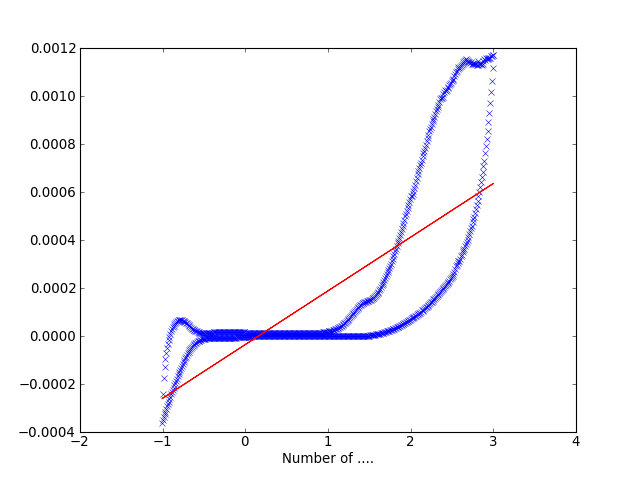
\includegraphics[scale=0.6]{../plots/test.png}
\end{center}
\end{figure}

\end{document}
